\problemname{Tivoli}
% TODO: include tivoli.png
% "Tivolit i exemplet med origo som ett blått kors och Lisas väg utritad. Den första anläggningen av varje attraktion är färgad rosa och den andra gul."
Lisa har kommit till tivolit och har bestämt vilka $N$ attraktioner hon vill åka, hon vill åka varje attraktion en gång.
För varje attraktion finns det två stycken anläggningar som är likvärdiga, det finns alltså totalt $2N$ anläggningar.
Givet positionerna för samtliga anläggninar, hjälp Lisa att planera vilka $N$ anläggningar hon ska välja och i vilken ordning för att minimera den sträcka hon måste gå för att ha åkt alla $N$ attraktioner.
Hon börjar dessutom vid entrén och ska också sluta där.
Entrén är vid origo.


I exemplet nedan är $N=3$ och anläggningarna för attraktion $a$ kallas $a_1$ och $a_2$.
Lisa går från entrén till $2_2$, sen till $1_1$, vidare till $3_1$ och slutligen tillbaka till entrén.
Den totala sträckan är $14{,}23345$.

\bigskip
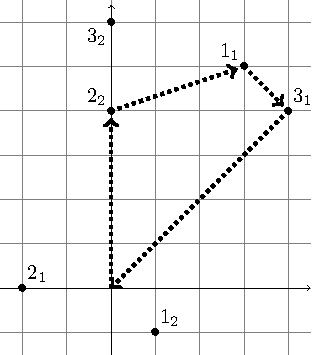
\includegraphics{img/tivoli-sample-img.pdf}

\section*{Indata}
Första raden består av heltalet $N$, antalet attraktioner Lisa vill åka ($1 \le N \le 15$).
Därefter följer $N$ rader, där den första raden beskriver attraktion nummer $1$, den andra raden attraktion nummer $2$ o.s.v.
Varje rad innehåller fyra heltal: x- och y-koordinat för den första anläggningen av denna attraktion, samt x- och y-koordinat för den andra anläggningen av denna attraktion.
Koordinaternas absolutbelopp understiger en miljon.

Ingen anläggning är på samma plats som en annan, eller på origo.

\section*{Utdata}
Den första raden av utdatan ska bestå av ett flyttal: hur långt Lisa måste gå.
Därefter ska $N$ rader följa med två heltal vardera, varav det första inom (mellan $1$ och $N$) säger vilken attraktion hon ska gå till, och det andra inom ($1$ eller $2$) vilken av anläggningarna.

Den första av dessa $N$ rader säger alltså vilken anläggning som hon först går till och den sista raden vilken anläggning hon sist går till.
Om det finns flera vägar som ger lika kort sträcka (det finns ju åtminstone alltid två håll att gå) kan du ange vilken som helst av dem.
Notera även att det första flyttalet som skrivs ut ska ta till hänsyn även att Lisa måste börja och sluta vid entrén.

Det relativa felet ska understiga $10^{-5}$.
